\textbf{GPSR (Greedy Perimeter Stateless Routing)}\cite{gpsr}は, 
位置情報を利用してパケットを転送する位置ベースの
ルーティングプロトコルであり, VANETのような動的かつ高速に変化する
ネットワーク環境に適している.
GPSRでは, 自身の位置やIPアドレスなどの情報をのせたHelloパケットを
一定間隔で隣接ノードに送信する.
図\ref{fig:nodetable}に示すように, それぞれのノードはIPアドレスや隣接ノードの
位置などの情報が記載された隣接ノードテーブルをもち, 
受信したHelloパケットの情報を用いて隣接ノードテーブルを
更新することにより, 周辺ノードの情報を把握する. 
この隣接ノードテーブルの情報をもとに, Greedy Forwarding と 
Perimeter Forwarding を組み合わせたルーティングプロトコルに従う. 

\begin{figure}
  \centering
  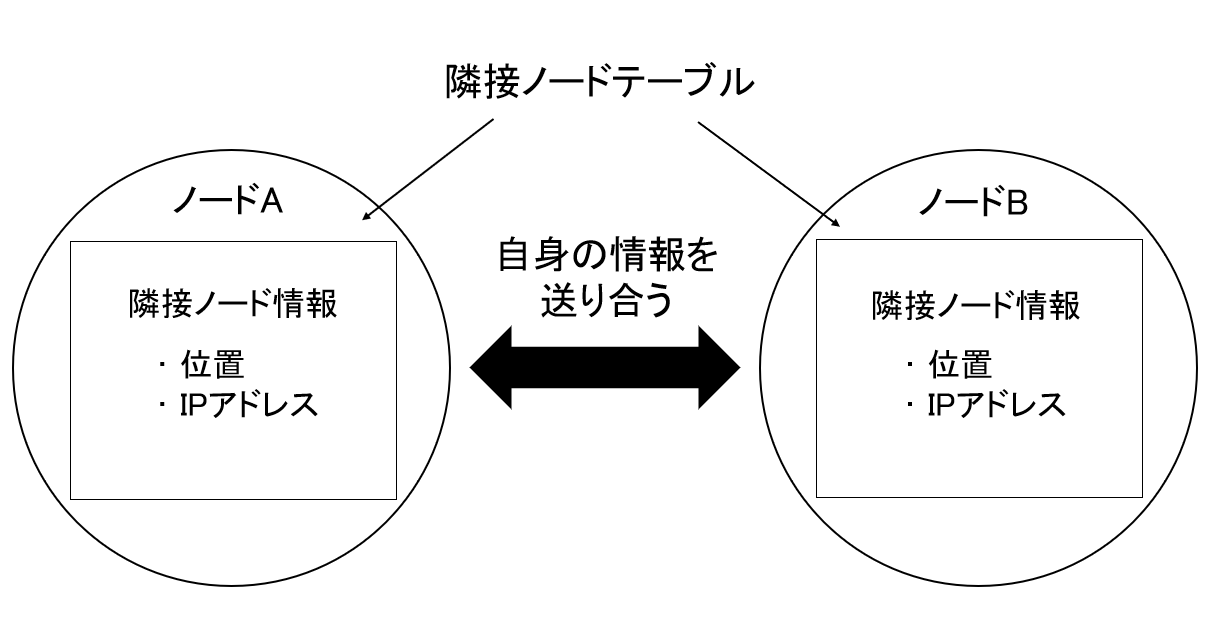
\includegraphics[scale=0.55]{figures/nodetable.png}
  \caption{GPSRの隣接ノードテーブル\cite{shinato}}
  \label{fig:nodetable}
\end{figure}

\noindent {\Large\textbf{Greedy Forwarding}}\\
\indent \textbf{Greedy Forwarding}はGPSRの基本的な
ルーティングプロトコルである. 図\ref{fig:greedy}に示すように, 
送信ノードSは, 宛先ノードDの位置情報をもとに
自身の電波伝搬範囲内のノードから, Dに最も近いノードを
ネクストホップとして選択する. 前提として, 送信ノードSは宛先ノードDの
位置情報を事前に把握しているものとする. 点線で書かれた円は全ノードの
受信感度が等しい場合の送信ノードSの電波伝搬範囲を, 
破線は宛先ノードとの距離を表している.

\begin{figure}
  \centering
  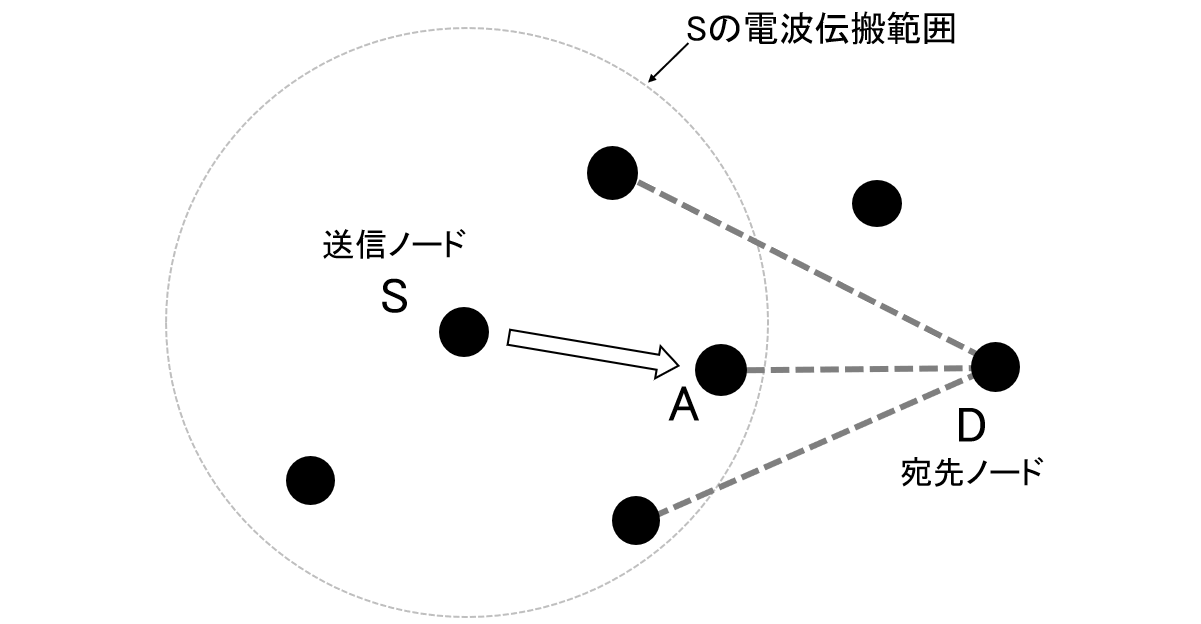
\includegraphics[scale=0.55]{figures/greedy.png}
  \caption{Greedy Forwarding\cite{shinato}}
  \label{fig:greedy}
\end{figure}

Greedy Forwardingでは局所最大問題と呼ばれる問題が生じてしまうことがある. 
\textbf{局所最大問題}とは, 図\ref{fig:local}に示すように, 送信ノードSの電波伝搬範囲内に
宛先ノードDが存在しない, かつ, 送信ノードSが自身の
電波伝搬範囲内で宛先ノードDに最も近い場合, 選択できる
ネクストホップが存在しなくなるという問題である.

\begin{figure}
  \centering
  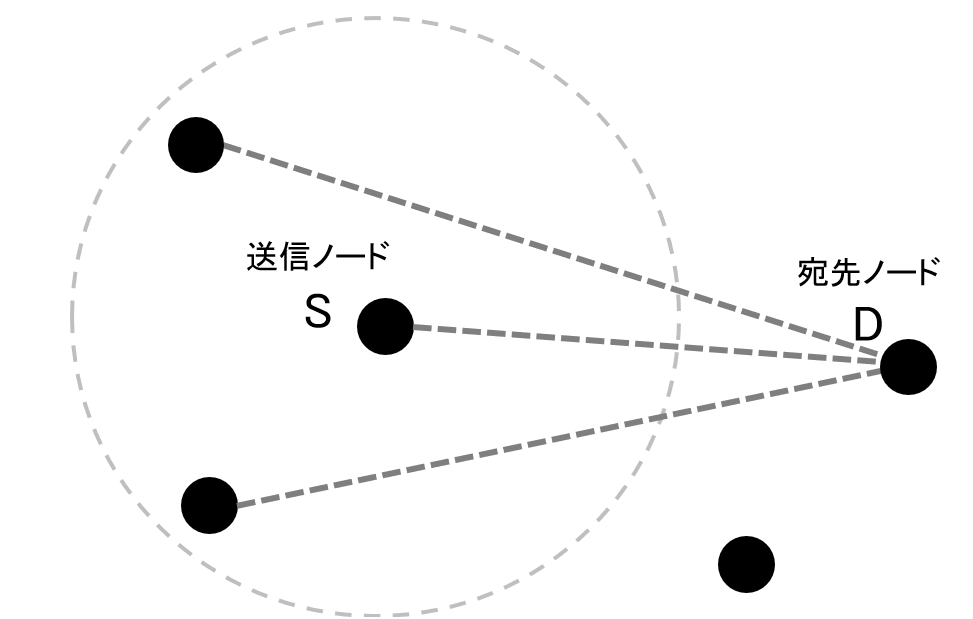
\includegraphics[scale=0.55]{figures/local.png}
  \caption{局所最大問題}
  \label{fig:local}
\end{figure}

\noindent {\Large\textbf{Perimeter Forwarding}}\\
Greedy Forwardingで局所最大問題が発生した場合に, 
Perimeter Forwardingが使用される. 
図1.5のように, 送信ノードSを中心に
\textbf{Right Hand Rule} に則って反時計回りにノードを探索し, 
最初に発見したノードをホップとして選択する方式である.

\textbf{図1.5を挿入}